\section{RDF}
\labsec{ch02-rdf}
Resource Description Framework (RDF) is a standard model for data interchange on the web, started in 1998 and the first version of the specification was published in 2004 by the W3C according to \sidecite{rdf-primer}. RDF has features that facilitate data merging even if the underlying schemas differ, and it specifically supports the evolution of schemas over time without requiring all the data consumers to be changed. Another important feature is that RDF supports XML, N-Triples and Turtle syntax, the \reffig{rdf-ntriples-ex} shows an example of how a triplet can be written in RDF N-Triples Syntax.

\begin{figure}[hb]
\begin{lstlisting}
<http://example/subject1> <http://example/predicate1> <http://example/object1>
\end{lstlisting}
\caption[RDF N-Triples Example]{RDF N-Triples Example. From this example we can see that each triplet is composed of three elements, the subject the predicate and the object.}
\labfig{rdf-ntriples-ex}
\end{figure}

RDF extends the linking structure of the Web to use URIs to name the relationship between things as well as the two ends of the link (this is usually referred to as a “triple” or "triplet"). Using this simple model, it allows structured and semi-structured data to be mixed, exposed, and shared across different applications. \reffig{rdf-graph} shows an example of how different triples can be use to compose a graph, this graph represents the same as the \reffig{rdf-ntriples-graph}

\begin{figure}[hb]
\begin{lstlisting}
<http://example/bob> <http://example/knows> <http://example/alice> .
<http://example/alice> <http://example/knows> <http://example/peter> .
\end{lstlisting}
\caption[RDF N-Triples Graph Example]{RDF N-Triples Graph Example. This exmaple shows the n-triples that generate the graph from \reffig{rdf-graph}.}
\labfig{rdf-ntriples-graph}
\end{figure}

This linking structure forms a directed, labeled graph, where the edges represent the named link between two resources, represented by the graph nodes. This graph view is the easiest possible mental model for RDF and is often used in easy-to-understand visual explanations.

Also, related to this we strongly recommend the Tim Berners-Lee’s writings on Web Design Issues \sidecite{semantic-roadmap} where he explain the issues of the liked data and why is RDF so important.

\begin{marginfigure}
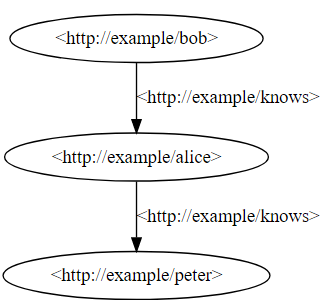
\includegraphics{rdf-graph}
\caption[RDF Example graph]{RDF Example graph.}
\labfig{rdf-graph}
\end{marginfigure}
